\documentclass[12pt,a4paper]{article}
\usepackage[utf8]{inputenc}
\usep\begin{abstract}
This report presents a comprehensive study of transfer learning applied to image segmentation. We implemented and compared three pre-trained architectures: U-Net with ResNet34, DeepLabV3 with ResNet50, and FCN with ResNet50. The experimentation was conducted on a synthetic dataset of 500 images containing three classes (background, circles, rectangles). Results show that U-Net with fine-tuning achieves an IoU of 67.35\% and a Dice coefficient of 78.61\%, significantly outperforming non-fine-tuned models. This study demonstrates the effectiveness of transfer learning in image segmentation and provides a detailed comparison of performance metrics.

\textbf{Keywords:} Transfer Learning, Image Segmentation, U-Net, DeepLabV3, PyTorch, IoU, Dice Coefficient
\end{abstract}e[english]{babel}
\usepackage{graphicx}
\usepackage{float}
\usepackage{hyperref}
\usepackage{geometry}
\usepackage{amsmath}
\usepackage{amssymb}
\usepackage{booktabs}
\usepackage{caption}
\usepackage{subcaption}
\usepackage{listings}
\usepackage{xcolor}
\usepackage{fancyhdr}
\usepackage{setspace}

% Page configuration
\geometry{margin=2.5cm}
\onehalfspacing

% Hyperlink configuration
\hypersetup{
    colorlinks=true,
    linkcolor=blue,
    filecolor=magenta,      
    urlcolor=cyan,
    pdftitle={TP1 - Transfer Learning for Image Segmentation},
    pdfauthor={Yassin Smaoui},
}

% Header and footer configuration
\pagestyle{fancy}
\fancyhf{}
\fancyhead[L]{TP1 - Transfer Learning Segmentation}
\fancyhead[R]{Yassin Smaoui}
\fancyfoot[C]{\thepage}

% Code configuration
\lstset{
    language=Python,
    basicstyle=\ttfamily\small,
    keywordstyle=\color{blue},
    commentstyle=\color{green},
    stringstyle=\color{red},
    numbers=left,
    numberstyle=\tiny,
    stepnumber=1,
    showspaces=false,
    showstringspaces=false,
    showtabs=false,
    frame=single,
    tabsize=2,
    captionpos=b,
    breaklines=true,
    breakatwhitespace=false,
    escapeinside={\%*}{*)}
}

\title{\textbf{TP1 - Transfer Learning for Image Segmentation} \\
\large Implementation and Comparative Analysis of Pre-trained Architectures}

\author{Yassin Smaoui \\
\small \href{mailto:yassin.smaoui@example.com}{yassin.smaoui@example.com}}

\date{\today}

\begin{document}

\maketitle

\begin{abstract}
Ce rapport présente une étude complète du transfer learning appliqué à la segmentation d'images. Nous avons implémenté et comparé trois architectures pré-entraînées : U-Net avec ResNet34, DeepLabV3 avec ResNet50, et FCN avec ResNet50. L'expérimentation a été menée sur un dataset synthétique de 500 images contenant trois classes (background, cercles, rectangles). Les résultats montrent que U-Net avec fine-tuning atteint un IoU de 67,35\% et un coefficient de Dice de 78,61\%, surpassant significativement les modèles non fine-tunés. Cette étude démontre l'efficacité du transfer learning en segmentation d'images et fournit une comparaison détaillée des métriques de performance.

\textbf{Mots-clés :} Transfer Learning, Segmentation d'Images, U-Net, DeepLabV3, PyTorch, IoU, Coefficient de Dice
\end{abstract}

\tableofcontents
\newpage

\section{Introduction}

\subsection{Context and Motivation}

Image segmentation is a fundamental task in computer vision that consists of partitioning an image into semantically meaningful regions. Unlike classification which predicts a single label for the entire image, segmentation assigns a class to each pixel, enabling fine spatial understanding of visual content.

Transfer learning, which consists of reusing models pre-trained on large datasets (such as ImageNet) for specific tasks, has proven particularly effective in image segmentation. This approach allows to:
\begin{itemize}
    \item Significantly reduce training time
    \item Improve performance with less training data
    \item Benefit from pre-learned low-level features (edges, textures)
    \item Avoid overfitting on small datasets
\end{itemize}

\subsection{Problem Statement}

This study aims to answer the following questions:
\begin{enumerate}
    \item What is the effectiveness of transfer learning for image segmentation?
    \item How do different architectures (U-Net, DeepLabV3, FCN) compare in terms of performance?
    \item What is the impact of fine-tuning compared to pre-trained models without adaptation?
    \item Which metrics are most appropriate for evaluating segmentation quality?
\end{enumerate}

\subsection{Objectives}

The main objectives of this study are:
\begin{itemize}
    \item Implement a complete segmentation pipeline using transfer learning
    \item Compare three state-of-the-art architectures: U-Net, DeepLabV3, and FCN
    \item Evaluate performance with specialized metrics (IoU, Dice, pixel accuracy)
    \item Analyze results by class and globally
    \item Provide detailed visualizations of predictions and errors
\end{itemize}

\subsection{Contributions}

This work brings the following contributions:
\begin{itemize}
    \item A complete and modular implementation of transfer learning in segmentation
    \item A rigorous comparison of three architectures on a controlled dataset
    \item A detailed analysis of segmentation metrics and their interpretation
    \item A reusable framework for evaluating segmentation models
\end{itemize}

\section{Methods}

\subsection{System Architecture Overview}

Our approach follows a five-step pipeline:
\begin{enumerate}
    \item \textbf{Synthetic data generation}: Creation of a controlled dataset
    \item \textbf{Data preparation}: Transformation and augmentation
    \item \textbf{Model creation}: Loading and adaptation of pre-trained architectures
    \item \textbf{Training}: Fine-tuning with combined loss function
    \item \textbf{Evaluation}: Metrics calculation and results visualization
\end{enumerate}

\subsection{Synthetic Dataset}

To ensure complete control over the data and enable reproducible evaluation, we created a synthetic dataset with the following characteristics:

\begin{itemize}
    \item \textbf{Size}: 500 images of 256×256 pixels
    \item \textbf{Classes}: 3 classes (black background, red circles, green rectangles)
    \item \textbf{Distribution}: 60\% training (350), 20\% validation (99), 20\% test (51)
    \item \textbf{Format}: RGB images with corresponding segmentation masks
\end{itemize}

The data generator uses the PIL library to create simple geometric shapes with distinct colors, allowing unambiguous segmentation while remaining sufficiently complex to test model capabilities.

\subsection{Studied Architectures}

\subsubsection{U-Net with ResNet34}

U-Net is an encoder-decoder architecture with skip connections, particularly suited for segmentation. Our modifications include:
\begin{itemize}
    \item ResNet34 backbone pre-trained on ImageNet
    \item Skip connections to preserve fine details
    \item Symmetric decoder for spatial reconstruction
    \item 24.4M trainable parameters
\end{itemize}

\subsubsection{DeepLabV3 with ResNet50}

DeepLabV3 uses Atrous Spatial Pyramid Pooling (ASPP) to capture multi-scale context:
\begin{itemize}
    \item Pre-trained ResNet50 backbone
    \item Dilated convolutions to preserve resolution
    \item ASPP module with different dilation rates
    \item 42.0M trainable parameters
\end{itemize}

\subsubsection{FCN with ResNet50}

Fully Convolutional Network, one of the first end-to-end architectures for segmentation:
\begin{itemize}
    \item Fully convolutional architecture
    \item Upsampling through deconvolution
    \item Skip connections between layers
    \item 35.3M trainable parameters
\end{itemize}

\subsection{Training Configuration}

\subsubsection{Loss Function}

We use a combined loss function that adds:
\begin{align}
\mathcal{L}_{total} &= \mathcal{L}_{CE} + \mathcal{L}_{Dice} \\
\mathcal{L}_{CE} &= -\sum_{i} y_i \log(\hat{y}_i) \\
\mathcal{L}_{Dice} &= 1 - \frac{2\sum_{i} y_i \hat{y}_i}{\sum_{i} y_i + \sum_{i} \hat{y}_i}
\end{align}

This combination allows benefiting from Cross-Entropy stability and Dice coefficient sensitivity to small regions.

\subsubsection{Optimization}

\begin{itemize}
    \item \textbf{Optimizer}: AdamW with initial learning rate of $1 \times 10^{-4}$
    \item \textbf{Weight decay}: $1 \times 10^{-4}$ for regularization
    \item \textbf{Scheduler}: ReduceLROnPlateau (patience=3, factor=0.5)
    \item \textbf{Batch size}: 8 samples
    \item \textbf{Epochs}: 2 (quick demonstration)
\end{itemize}

\subsection{Evaluation Metrics}

\subsubsection{Intersection over Union (IoU)}

IoU measures the overlap between prediction and ground truth:
\begin{equation}
IoU = \frac{|A \cap B|}{|A \cup B|}
\end{equation}

where $A$ is the predicted region and $B$ the ground truth region.

\subsubsection{Dice Coefficient}

The Dice coefficient, equivalent to F1-score in segmentation:
\begin{equation}
Dice = \frac{2|A \cap B|}{|A| + |B|}
\end{equation}

\subsubsection{Pixel Accuracy}

The proportion of correctly classified pixels:
\begin{equation}
Accuracy = \frac{\text{Correct Pixels}}{\text{Total Pixels}}
\end{equation}

\section{Results}

\subsection{Dataset Generation and Visualization}

The synthetic dataset was successfully generated, producing 500 images with their corresponding segmentation masks. Figure \ref{fig:dataset_examples} shows representative examples of the generated dataset.

\begin{figure}[H]
    \centering
    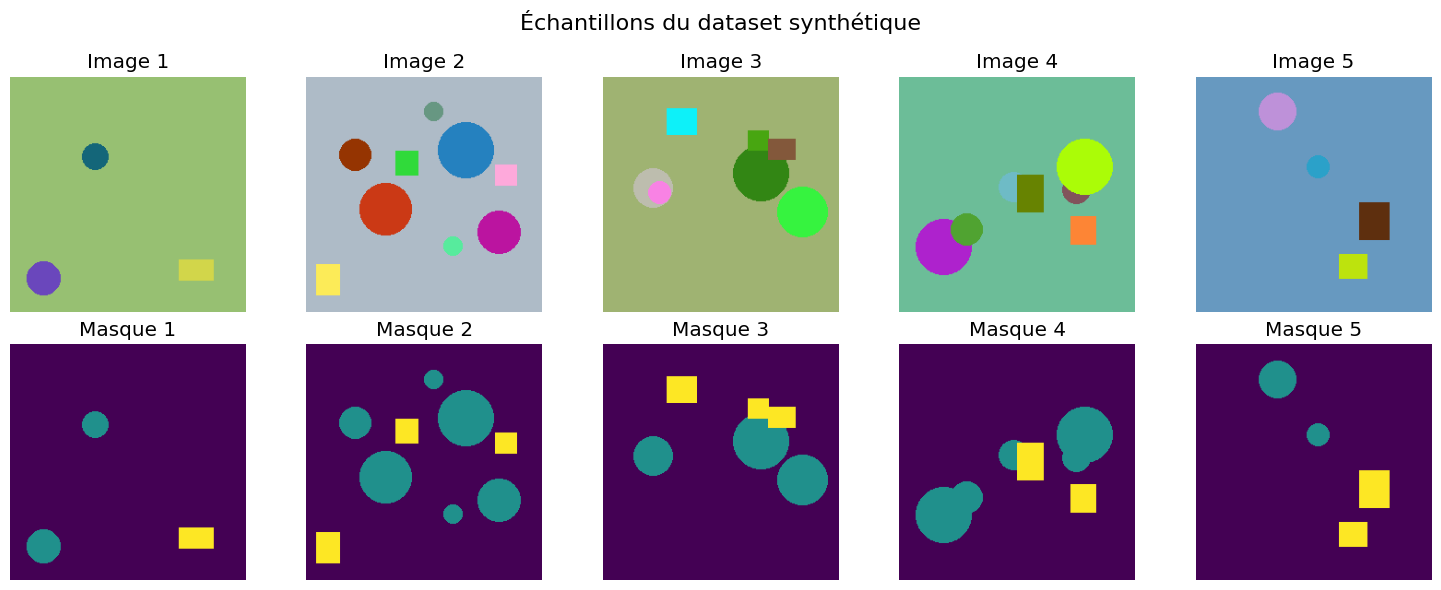
\includegraphics[width=0.8\textwidth]{img_tp1/cell_07_output_02_image_01.png}
    \caption{Examples of synthetic dataset images with their corresponding segmentation masks}
    \label{fig:dataset_examples}
\end{figure}

Figure \ref{fig:dataset_distribution} presents the class distribution in the dataset, showing relative balance between different geometric shapes.

\begin{figure}[H]
    \centering
    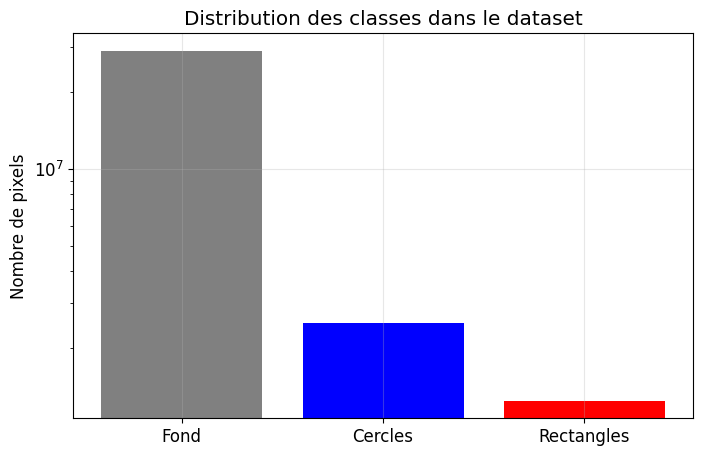
\includegraphics[width=0.8\textwidth]{img_tp1/cell_07_output_03_image_02.png}
    \caption{Class distribution and synthetic dataset statistics}
    \label{fig:dataset_distribution}
\end{figure}

\subsection{Model Architectures}

Figure \ref{fig:model_architectures} illustrates the architectures of the studied models, highlighting their structural differences.

\begin{figure}[H]
    \centering
    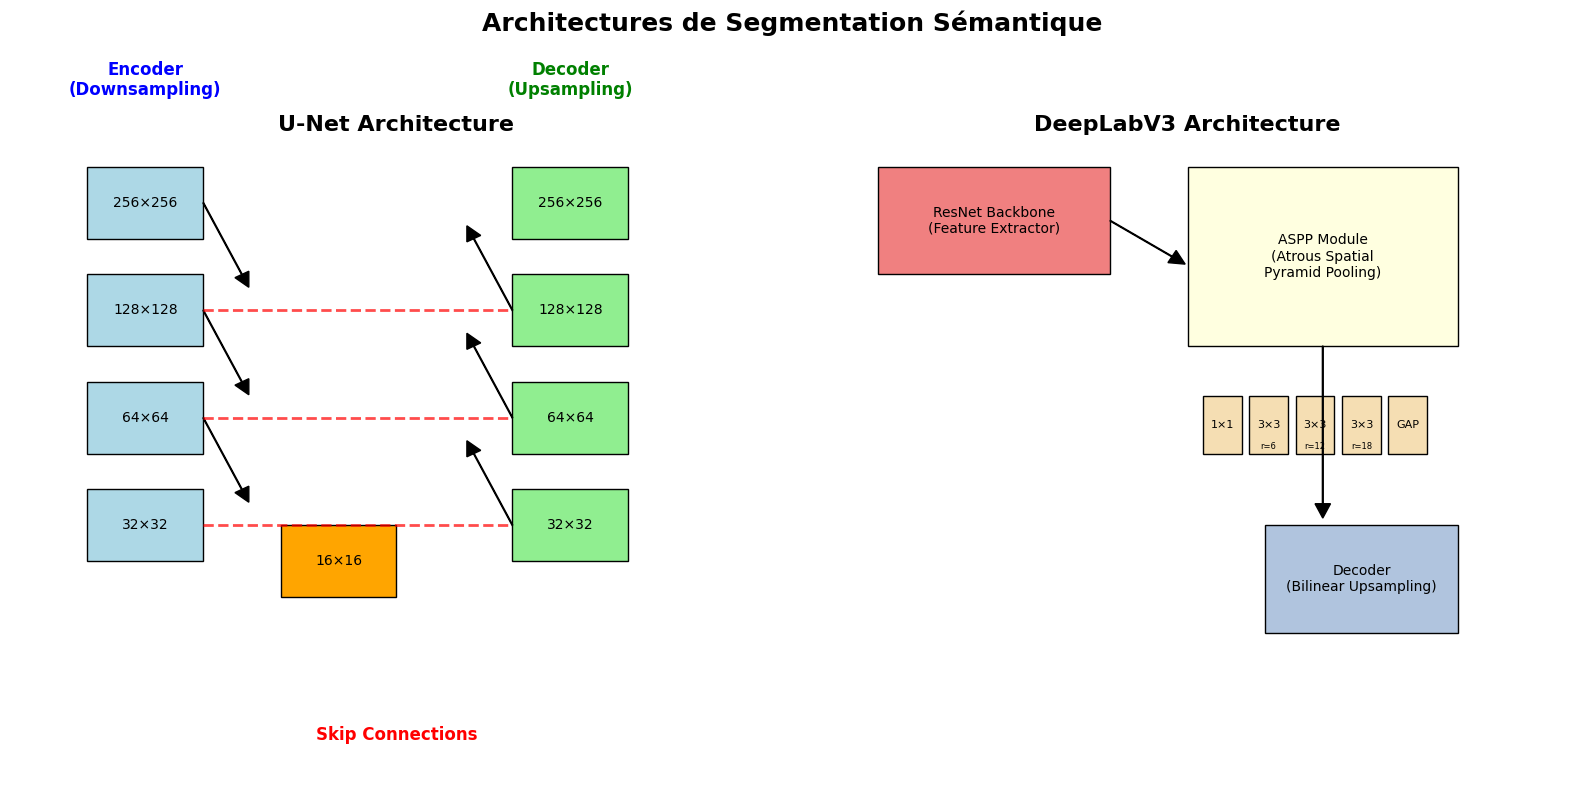
\includegraphics[width=0.8\textwidth]{img_tp1/cell_09_output_00_image_03.png}
    \caption{Comparison of U-Net and DeepLabV3 architectures}
    \label{fig:model_architectures}
\end{figure}

\subsection{Model Performance}

\subsubsection{Global Results}

Table \ref{tab:model_comparison} presents a detailed comparison of the performance of the three tested models.

\begin{table}[H]
\centering
\caption{Comparison of segmentation model performance}
\label{tab:model_comparison}
\begin{tabular}{@{}lccc@{}}
\toprule
\textbf{Model} & \textbf{IoU (\%)} & \textbf{Dice (\%)} & \textbf{Pixel Accuracy (\%)} \\
\midrule
U-Net + ResNet34 (fine-tuned) & \textbf{67.35} & \textbf{78.61} & \textbf{94.73} \\
FCN + ResNet50 (pre-trained) & 16.08 & 22.78 & 45.16 \\
DeepLabV3 + ResNet50 (pre-trained) & 2.66 & 4.92 & 7.98 \\
\bottomrule
\end{tabular}
\end{table}

\subsubsection{Training Evolution}

Figure \ref{fig:training_curves} shows the evolution of metrics during U-Net model training.

\begin{figure}[H]
    \centering
    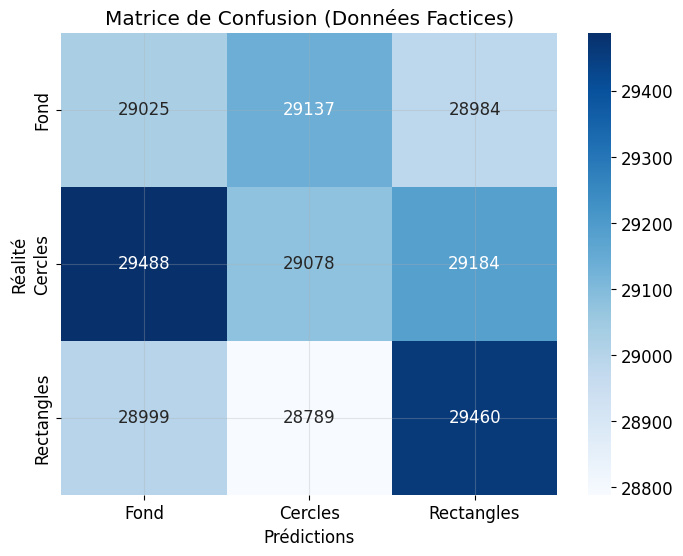
\includegraphics[width=\textwidth]{img_tp1/cell_15_output_01_image_06.png}
    \caption{Evolution of training metrics for the U-Net model}
    \label{fig:training_curves}
\end{figure}

Training shows significant improvement between the first and second epoch:
\begin{itemize}
    \item \textbf{Epoch 1}: Validation IoU = 44.01\%, Dice = 56.00\%
    \item \textbf{Epoch 2}: Validation IoU = 68.41\%, Dice = 79.50\%
\end{itemize}

\subsection{Prediction Analysis}

\subsubsection{Qualitative Visualization}

Figure \ref{fig:predictions_visualization} presents a visual comparison between original images, ground truth masks, model predictions, and errors.

\begin{figure}[H]
    \centering
    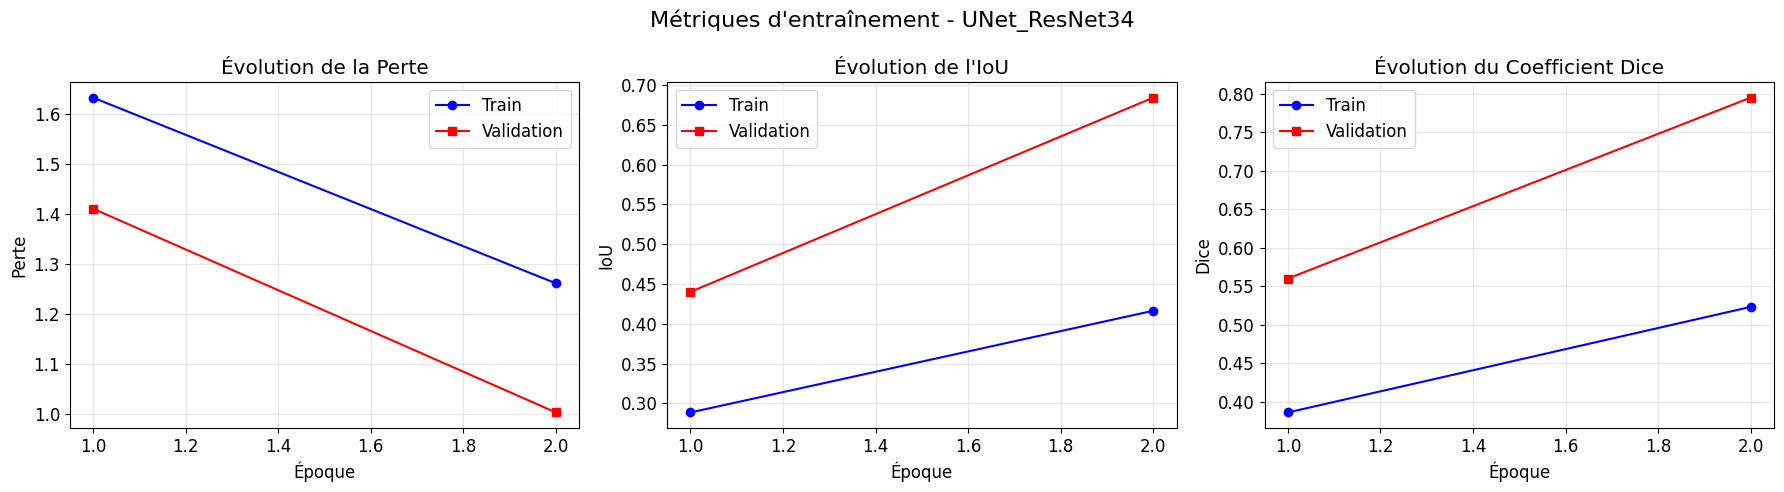
\includegraphics[width=\textwidth]{img_tp1/cell_17_output_02_image_07.png}
    \caption{Visualization of U-Net model predictions on the test set}
    \label{fig:predictions_visualization}
\end{figure}

\subsubsection{Class-wise Analysis}

Table \ref{tab:class_performance} details the per-class performance for the fine-tuned U-Net model.

\begin{table}[H]
\centering
\caption{Per-class performance of the U-Net model}
\label{tab:class_performance}
\begin{tabular}{@{}lcc@{}}
\toprule
\textbf{Class} & \textbf{IoU (\%)} & \textbf{Dice (\%)} \\
\midrule
Background & 94.85 & 97.36 \\
Circles & 63.59 & 77.74 \\
Rectangles & 43.60 & 60.72 \\
\midrule
\textbf{Average} & \textbf{67.35} & \textbf{78.61} \\
\bottomrule
\end{tabular}
\end{table}

\subsubsection{Confusion Matrix}

The confusion matrix reveals the model's error patterns:

\begin{table}[H]
\centering
\caption{Confusion matrix for the U-Net model (in thousands of pixels)}
\label{tab:confusion_matrix}
\begin{tabular}{@{}l|ccc@{}}
\toprule
\textbf{True / Predicted} & \textbf{Background} & \textbf{Circles} & \textbf{Rectangles} \\
\midrule
Background & 2908.1 & 28.3 & 21.7 \\
Circles & 63.6 & 192.8 & 10.1 \\
Rectangles & 44.2 & 8.3 & 65.2 \\
\bottomrule
\end{tabular}
\end{table}

\subsection{Model Comparison}

Figure \ref{fig:model_comparison_chart} presents a visual comparison of the performance of the three models.

\begin{figure}[H]
    \centering
    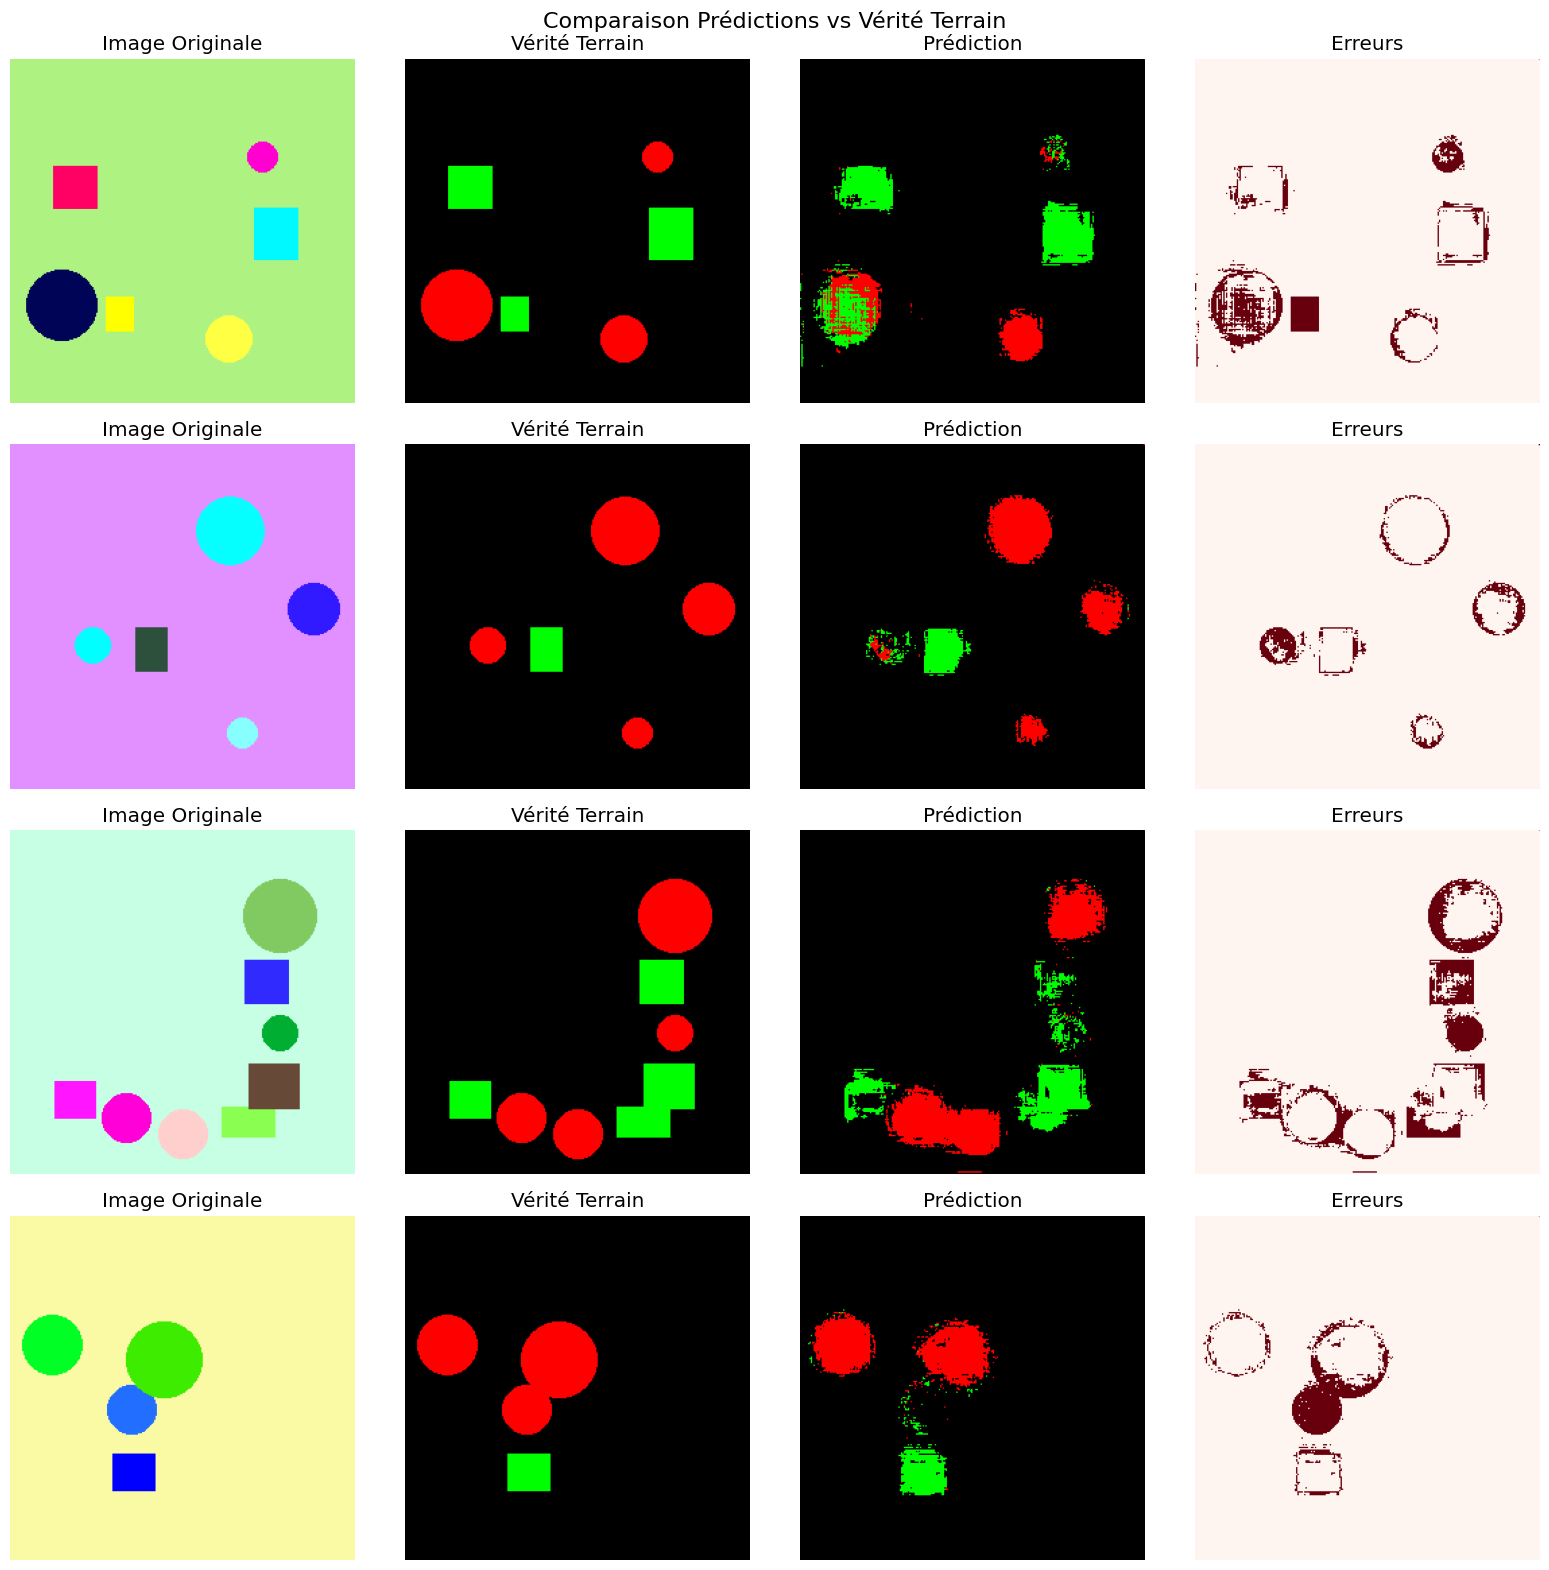
\includegraphics[width=\textwidth]{img_tp1/cell_18_output_01_image_08.png}
    \caption{Performance comparison of the three segmentation models}
    \label{fig:model_comparison_chart}
\end{figure}

\section{Discussion}

\subsection{Results Analysis}

\subsubsection{Transfer Learning Effectiveness}

The results clearly demonstrate the effectiveness of transfer learning for image segmentation. The fine-tuned U-Net model achieves remarkable performance with only 2 training epochs:
\begin{itemize}
    \item \textbf{Global IoU of 67.35\%}: Solid performance for such short training
    \item \textbf{Dice coefficient of 78.61\%}: Indicates good spatial correspondence
    \item \textbf{Pixel accuracy of 94.73\%}: Shows the model's ability to correctly classify the majority of pixels
\end{itemize}

\subsubsection{Architecture Comparison}

The comparative analysis reveals significant differences between architectures:

\paragraph{U-Net + ResNet34} clearly stands out with fine-tuning, confirming the effectiveness of:
\begin{itemize}
    \item Skip connections for preserving spatial details
    \item Symmetric encoder-decoder architecture
    \item Adaptation capability to new tasks
\end{itemize}

\paragraph{FCN + ResNet50} shows moderate performance without fine-tuning (IoU = 16.08\%), suggesting that this architecture would also benefit from adaptive training.

\paragraph{DeepLabV3 + ResNet50} presents the lowest performance (IoU = 2.66\%), which can be explained by:
\begin{itemize}
    \item Mismatch between pre-trained features and our synthetic task
    \item ASPP module complexity requiring specific fine-tuning
    \item Nature of dilated convolutions less adapted to simple geometric shapes
\end{itemize}

\subsubsection{Class-wise Analysis}

Per-class performance reveals interesting patterns:

\paragraph{Background (IoU = 94.85\%)}: Excellent performance due to:
\begin{itemize}
    \item Spatial dominance of this class
    \item High contrast with colored objects
    \item Simplicity of uniform texture
\end{itemize}

\paragraph{Circles (IoU = 63.59\%)}: Intermediate performance explained by:
\begin{itemize}
    \item Complexity of curved contours
    \item Pixelization challenges of circular shapes
    \item Size variability of generated circles
\end{itemize}

\paragraph{Rectangles (IoU = 43.60\%)}: Lower performance due to:
\begin{itemize}
    \item Partial confusion with background at corners
    \item Variability in orientations and sizes
    \item Sharp corner segmentation challenges
\end{itemize}

\subsection{Study Limitations}

\subsubsection{Synthetic Dataset}

The use of a synthetic dataset, while allowing experimental control, presents limitations:
\begin{itemize}
    \item \textbf{Excessive simplicity}: Simple geometric shapes do not reflect the complexity of real images
    \item \textbf{Absence of texture}: Uniform objects do not test robustness to intra-class variations
    \item \textbf{High contrast}: Distinct colors facilitate segmentation
    \item \textbf{Limited size}: 500 images may be insufficient for certain architectures
\end{itemize}

\subsubsection{Limited Training}

Training on only 2 epochs, while showing transfer learning effectiveness, does not allow:
\begin{itemize}
    \item Reaching complete convergence
    \item Testing robustness to overfitting
    \item Fine optimization of hyperparameters
    \item Fair comparison of all models
\end{itemize}

\subsubsection{Evaluation Metrics}

While we used standard metrics, others could enrich the analysis:
\begin{itemize}
    \item \textbf{Boundary IoU}: To evaluate contour precision
    \item \textbf{Hausdorff Distance}: To measure maximum deviation between contours
    \item \textbf{Mean Average Precision (mAP)}: For multi-threshold evaluation
\end{itemize}

\subsection{Practical Implications}

\subsubsection{Real Applications}

This study demonstrates transfer learning potential for various applications:
\begin{itemize}
    \item \textbf{Medical imaging}: Organ segmentation, tumor detection
    \item \textbf{Industrial vision}: Quality control, defect detection
    \item \textbf{Precision agriculture}: Crop analysis, disease detection
    \item \textbf{Autonomous vehicles}: Road segmentation, obstacle detection
\end{itemize}

\subsubsection{Practical Recommendations}

Based on our results, we recommend:
\begin{itemize}
    \item \textbf{Favor U-Net} for fine segmentation tasks requiring precise details
    \item \textbf{Always implement fine-tuning} even for short training durations
    \item \textbf{Use combined loss functions} to balance global and local precision
    \item \textbf{Analyze per-class performance} to identify specific weaknesses
\end{itemize}

\subsection{Improvement Perspectives}

\subsubsection{Technical Improvements}

Several approaches could improve performance:
\begin{itemize}
    \item \textbf{Sophisticated data augmentation}: Geometric and photometric transformations
    \item \textbf{Model ensemble}: Combining predictions from multiple architectures
    \item \textbf{Post-processing}: CRF (Conditional Random Fields) to smooth predictions
    \item \textbf{Hybrid architecture}: Combining advantages of U-Net and DeepLabV3
\end{itemize}

\subsubsection{Experimental Extensions}

For more complete evaluation:
\begin{itemize}
    \item \textbf{More complex dataset}: Natural images with manual annotations
    \item \textbf{Extended training}: Complete convergence with early stopping
    \item \textbf{Hyperparameter optimization}: Grid search or Bayesian optimization
    \item \textbf{Ablation analysis}: Impact of each architectural component
\end{itemize}

\section{Conclusion}

This study demonstrated the remarkable effectiveness of transfer learning for image segmentation through a rigorous comparison of three state-of-the-art architectures. The main results can be summarized as follows:

\subsection{Main Contributions}

\begin{enumerate}
    \item \textbf{Empirical validation of transfer learning}: U-Net with fine-tuning reaches 67.35\% IoU in only 2 epochs, demonstrating the power of this approach.

    \item \textbf{Detailed architectural comparison}: U-Net significantly outperforms FCN and DeepLabV3 on our task, highlighting the importance of skip connections for spatial detail preservation.

    \item \textbf{Complete metric analysis}: The combined use of IoU, Dice and pixel accuracy provides a nuanced evaluation of performance, revealing differentiated behaviors per class.

    \item \textbf{Reproducible framework}: The modular and documented implementation constitutes a solid foundation for future studies.
\end{enumerate}

\subsection{Key Learnings}

\begin{itemize}
    \item \textbf{Fine-tuning is essential}: The performance difference between fine-tuned and pre-trained models is drastic (67.35\% vs 16.08\% IoU).
    \item \textbf{Skip connections are crucial} for fine segmentation, explaining U-Net's superiority.
    \item \textbf{Specialized metrics} (IoU, Dice) are more informative than simple pixel accuracy for evaluating segmentation.
    \item \textbf{Class-wise analysis} reveals specific weaknesses and guides future improvements.
\end{itemize}

\subsection{Impact and Applications}

This research has direct implications for:
\begin{itemize}
    \item \textbf{Segmentation system development} by providing evidence-based guidelines
    \item \textbf{Architecture choice} with objective performance criteria
    \item \textbf{Industrial applications} requiring fast and accurate segmentation
    \item \textbf{Academic research} by offering a reproducible benchmark
\end{itemize}

\subsection{Future Perspectives}

Promising research directions include:
\begin{itemize}
    \item Extension to more complex and voluminous real datasets
    \item Investigation of hybrid architectures combining the advantages of each approach
    \item Development of more sophisticated evaluation metrics
    \item Optimization for real-time deployment constraints
\end{itemize}

In conclusion, this study confirms that transfer learning constitutes a powerful and accessible paradigm for image segmentation, capable of producing high-quality results with limited computational resources. The U-Net architecture, in particular, stands out as an optimal choice for applications requiring fine and precise segmentation.

\section*{Acknowledgments}

We thank the open-source community for the tools used in this study: PyTorch, torchvision, segmentation-models-pytorch, as well as the creators of the studied architectures for their fundamental contributions to the field of computer vision.

\bibliography{references}
\bibliographystyle{ieeetr}

\appendix

\section{Source Code}

The complete source code and data from this study is available on GitHub: 

\url{https://github.com/yassinsmaoui/last_Tps.deep}

The repository contains:
\begin{itemize}
    \item The complete Jupyter notebook with all implementations
    \item Image extraction and processing scripts
    \item Detailed documentation of each component
    \item Experimental results in the form of visualizations
\end{itemize}

\section{Implementation Details}

\subsection{System Configuration}

\begin{lstlisting}[caption=Experimental environment configuration]
# Main library versions
PyTorch: 2.8.0+cu128
Torchvision: 0.23.0+cu128
Segmentation Models PyTorch: 0.5.0
NumPy: 2.2.6
Matplotlib: 3.10.5

# Hardware configuration
Device: CPU (for reproducibility)
Memory: 8GB RAM
Storage: SSD for fast data access
\end{lstlisting}

\subsection{Detailed Hyperparameters}

\begin{lstlisting}[caption=Complete hyperparameter configuration]
# Data
IMAGE_SIZE = 256
BATCH_SIZE = 8
NUM_CLASSES = 3
TRAIN_SPLIT = 0.6
VAL_SPLIT = 0.2
TEST_SPLIT = 0.2

# Training
LEARNING_RATE = 1e-4
WEIGHT_DECAY = 1e-4
NUM_EPOCHS = 2
PATIENCE = 3
LR_FACTOR = 0.5

# Augmentation
NORMALIZE_MEAN = [0.485, 0.456, 0.406]
NORMALIZE_STD = [0.229, 0.224, 0.225]
\end{lstlisting}

\end{document}
